\documentclass[conference]{IEEEtran}
\usepackage{cite}
\usepackage{amsmath}
\ifCLASSINFOpdf
  \usepackage[pdftex]{graphicx}
   \DeclareGraphicsExtensions{.pdf,.jpeg,.png}
\else
 \fi
 
% correct bad hyphenation here
\hyphenation{op-tical net-works semi-conduc-tor}


\begin{document}
%
% paper title
% can use linebreaks \\ within to get better formatting as desired
% Do not put math or special symbols in the title.
\title{Dynamic Rendezvous based Routing Algorithm on Sparse Opportunistic Network Environment}


% author names and affiliations
% use a multiple column layout for up to three different
% affiliations
\author{\IEEEauthorblockN{Jiradett Kerdsri}
\IEEEauthorblockA{School of Information, Computer, \\and Communication Technology (ICT), \\Sirindhorn International Institute of Technology, Thailand
%\IEEEauthorblockA{ Defense Technology Institute \\(Public Organisation) Ministry of Defense, \\Nontburi, Thailand
\\Email: jiradett.k@dti.or.th}
\and
\IEEEauthorblockN{Komwut Wipusitwarkun}
\IEEEauthorblockA{School of Information, Computer, \\and Communication Technology (ICT), \\Sirindhorn International Institute of Technology, Thailand
\\Email: komwut@siit.tu.ac.th}
}

% make the title area
\maketitle

% As a general rule, do not put math, special symbols or citations
% in the abstract
\begin{abstract}
Opportunistic network is a challenge network where the nodes need to communicate with each other even either direct or indirect routes between them may not permanently exist due to the nodes' random movement.
Most routing algorithms in this dynamic network environment employ \textit{store-carry-forward} paradigm by which a node can keep the receiving messages, carrying the messages with them when moving and then forwarding the messages (or the copies) to the opportunistic meeting nodes when possible.
This routing model works well in the networks with high-to-moderate node density in which the opportunity that the moving nodes can meet with each other is rather high.
On the other hand, it has been reported that the delivery ratio becomes remarkably low in the sparse network environment especially when there is strict constraint on message delivery deadline.
In this paper, we introduce the novel concept of rendezvous place where the passing nodes can announce, deposit or pickup their own messages without having to meet the other nodes carrying the desired message. 
In the proposed scheme, the rendezvous place can be detected automatically and its area's size and shape are dynamically changed according to the interaction among nodes passing around the area.
The results from intensive simulations show that our proposed routing algorithm can achieve higher delivery ratio and utilize lower energy consumption than traditional opportunistic routing algorithms especially in sparse network environment.

\end{abstract}
\IEEEpeerreviewmaketitle



\section{Introduction}
%What is OppNet?
Opportunistic Network (OppNet) is an extreme type of Delay Tolerant Networks (DTNs) where the source and destination nodes might never be fully connected at the same time, thus there is no guarantee on the existence of a complete path between two nodes wishing to communicate \cite{MWNsBook2011}.
This intermittent connections may result from several factors such as high node mobility, low node density, environmental interference and obstruction, short radio range and malicious attacks \cite{prodhan2011} etc.
The node movement in OppNet is extremely random in some networking environment, thus the probability of message delivery from source to destination is difficult to assure.
Example of such networks are sparse mobile ad hoc network \cite{Alekeish2012}, military tactical networks \cite{Scott2005,Kerdsri2013}  or sensor networks, such as ZebraNet \cite{zebranet2004}, SWIM \cite{Small2003}  which are wireless sensor networks in which nodes move throughout an environment working to gather and process information about their surroundings.
Commonly, the key differentiating factors among those scenarios are the amount of predictability and control over the contacts between the message carriers\cite{Karkkainen2013}.
%Algorithms --> Store Carry Forward
A key concept behind Opportunistic Routing (OR) is overhearing and cooperation among relaying nodes to overcome the drawback of unreliable wireless transmission \cite{Liu2009}.
Since the mobile nodes are not always connected to each other, the forwarding algorithms in such network commonly follow a store-carry-forward (SCF) paradigm.
This SCF employs storage space and node mobility to overcome the intermittent connectivity \cite{Ma2011}.
The messages sent from the source node are carried by intermediate nodes to other geographical area and transfered to adjacent nodes until the destination node receives this message.
%From part A
Since this fundamental SCF routing model realistically requires a certain sufficient occasion of \emph{direct} encounter among moving nodes to exchange messages, its routing performance will highly degrade in the low-node-density sparse network \cite{Spyropoulos2010}.
%From part A2
Although there are several existing OppNet routing solutions \cite{ Zhang2013, Chung-Ming2008, Spyropoulos2004, Grossglauser2002, Vahdat2000,Kerdsri2013} proposed in the literature, very few proposals address the problem in this sparse network environment especially when the OppNet nodes are energy-constrained \cite{Liguang2013,Eu2010} and the direction of their movement cannot be controlled.
One interesting application of such OppNet environment is the sensor OppNet for wildlife monitoring and tracking \cite{zebranet2004, Small2003}.

%From part B
In this paper, we proposed a novel Dynamic Rendezvous based Routing Algorithms (DRRA) to increase message exchanging opportunity even in the sparse network environment.
We utilize the fact that there should be some node-gathering (Rendezvous) places forming somewhere at some specific time in the real network.
These Rendezvous places may be either predictable such as along the river in the wildlife monitoring application, or non-predictable such as disaster and emergency networks.
An energy constrained node should maximize its resource usage to communicate with the others only when entering into the rendezvous area.
In the proposed scheme, the rendezvous place is dynamically marked by the help of a special controllable Rendezvous node and the proposed rumor protocol to let nodes in the rendezvous area exchange messages more efficiently without having to directly meet with the other nodes.

The rest of the paper is organized as follows. 
In section II, we discuss the  overview of SFC routing models and existing works. 
The detail of rendezvous based routing model is elaborated in section III.
In section IV, we present the result of our simulation and show the performance of our scheme under different conditions.
We conclude the paper and point out some future research directions in section V.   


\section{The SCF routing models and existing works}
\begin{figure}[!t]
	\centering
	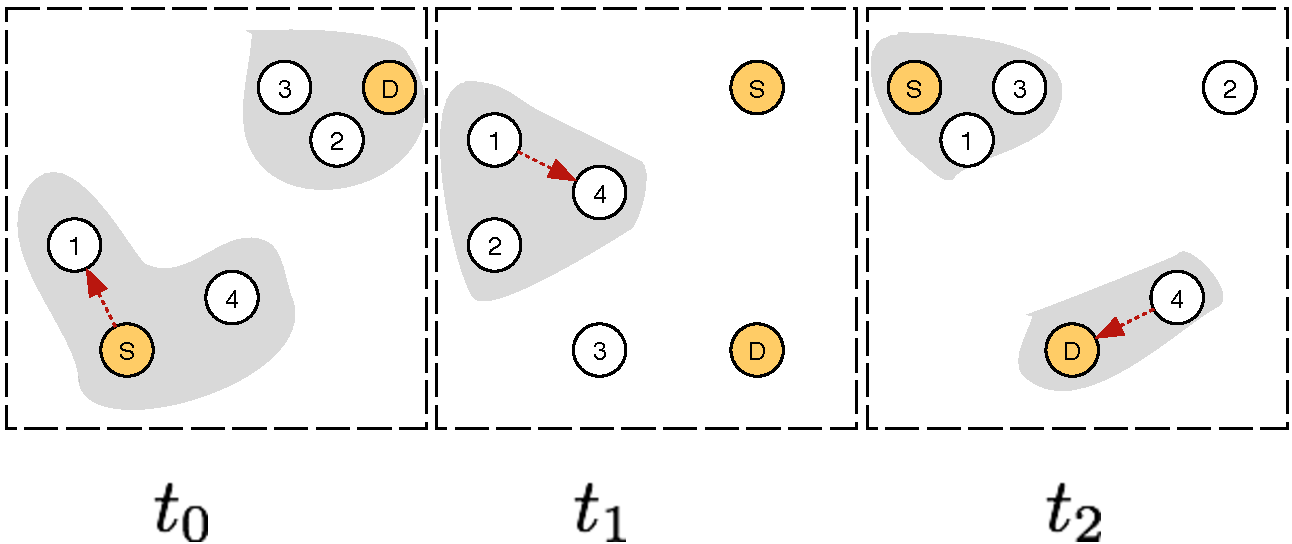
\includegraphics[width=3in]{Figures/SFC.pdf}
	\caption{Store Carry and Forward routing model}
	\label{SFC}
\end{figure}

In OppNet, the messages are delivered using Store-Carry-Forward routing by which  the nodes can exchange data whenever they come in close.
If there is no direct connection from source to destination, data holding nodes will discover their nearest neighbor nodes to forward messages toward the destination node as shown in Fig. \ref{SFC}.
There are several existing works in the literature \cite{Vahdat2000, Harras2005, Neena2013, Lindgren2003,Brendan2005,Boldrini2007,Kerdsri2013} with the aim for 100\% delivery ratio which is quite difficult to achieve especially in sparse network with constraints in energy consumption and message delivery deadline.

Vahdat et al \cite{Vahdat2000} proposed the epidemic routing using  uncontrolled flooding algorithm in which the replication of source data is not restricted with any limits in order to route the message from source to destination in the intermittently connected network.
However, this type of routing incurs significant demand on both bandwidth and buffer.
To address the excess traffic overhead, Khaled et al \cite{Harras2005} proposed a Controlled Flooding  scheme which can limit the flooding by three parameters: Willingness probability, Time-to-Live, and Kill Time.
Nevertheless, flooding based routing performance degrading has been reported in a very sparse network \cite{Neena2013}.

Lindgren et al \cite{Lindgren2003} proposed a prediction based routing called PROPHET (Probabilistic Routing Protocol using History of Encounters and Transitivity) by estimating the delivery predictability to indicate the probability of success in delivering a message to the destination from the local node.
In this prediction based routing category, Brun et al \cite{Brendan2005}  also proposed a protocol utilizing the motion vector of mobile nodes to predict the future location of mobile nodes by using the knowledge of relative velocities of a node and its neighbor nodes to predict the closest distance between two nodes.
Although the prediction based approach can reduce traffic overhead in the network, but it lacks of the aim to improve the performance in extremely low node density and failed in some certain cases which leads to the delivery ratio reduction.

To refine the prediction based routing,  Boldrini et al \cite{Boldrini2007}  proposed the History based routing (HiBOp) which exploits current context information for data forwarding decisions.
Even though, this context based routing approach can reduce the resource consumption in terms of network traffic and storage but it increases the delay which results in significantly less efficient than Epidemic algorithm.
%In our work of content based routing, DORSI protocol \cite{Kerdsri2013} aims to differentiate the messages by their significant in order to improve the delivery ration of important data.
Kerdsri et al \cite{Kerdsri2013} proposed DORSI protocol with the concept of content based routing which aims to classify the data in the network by messages' significance level in order to guarantee the delivery of more important data. 
However, the decreasing in network performance under sparse environment is not mentioned in this proposed protocol.
Overall, the performance of most existing algorithms are degrading in very sparse node density and the energy consumption does not take in to the consideration which is a crucial factor in such mobile sensor devices such as in wildlife monitoring.


\section{The proposed Rendezvous based OppNet system}

\subsection{System model}
\begin{figure*}[!t]
	\centering
	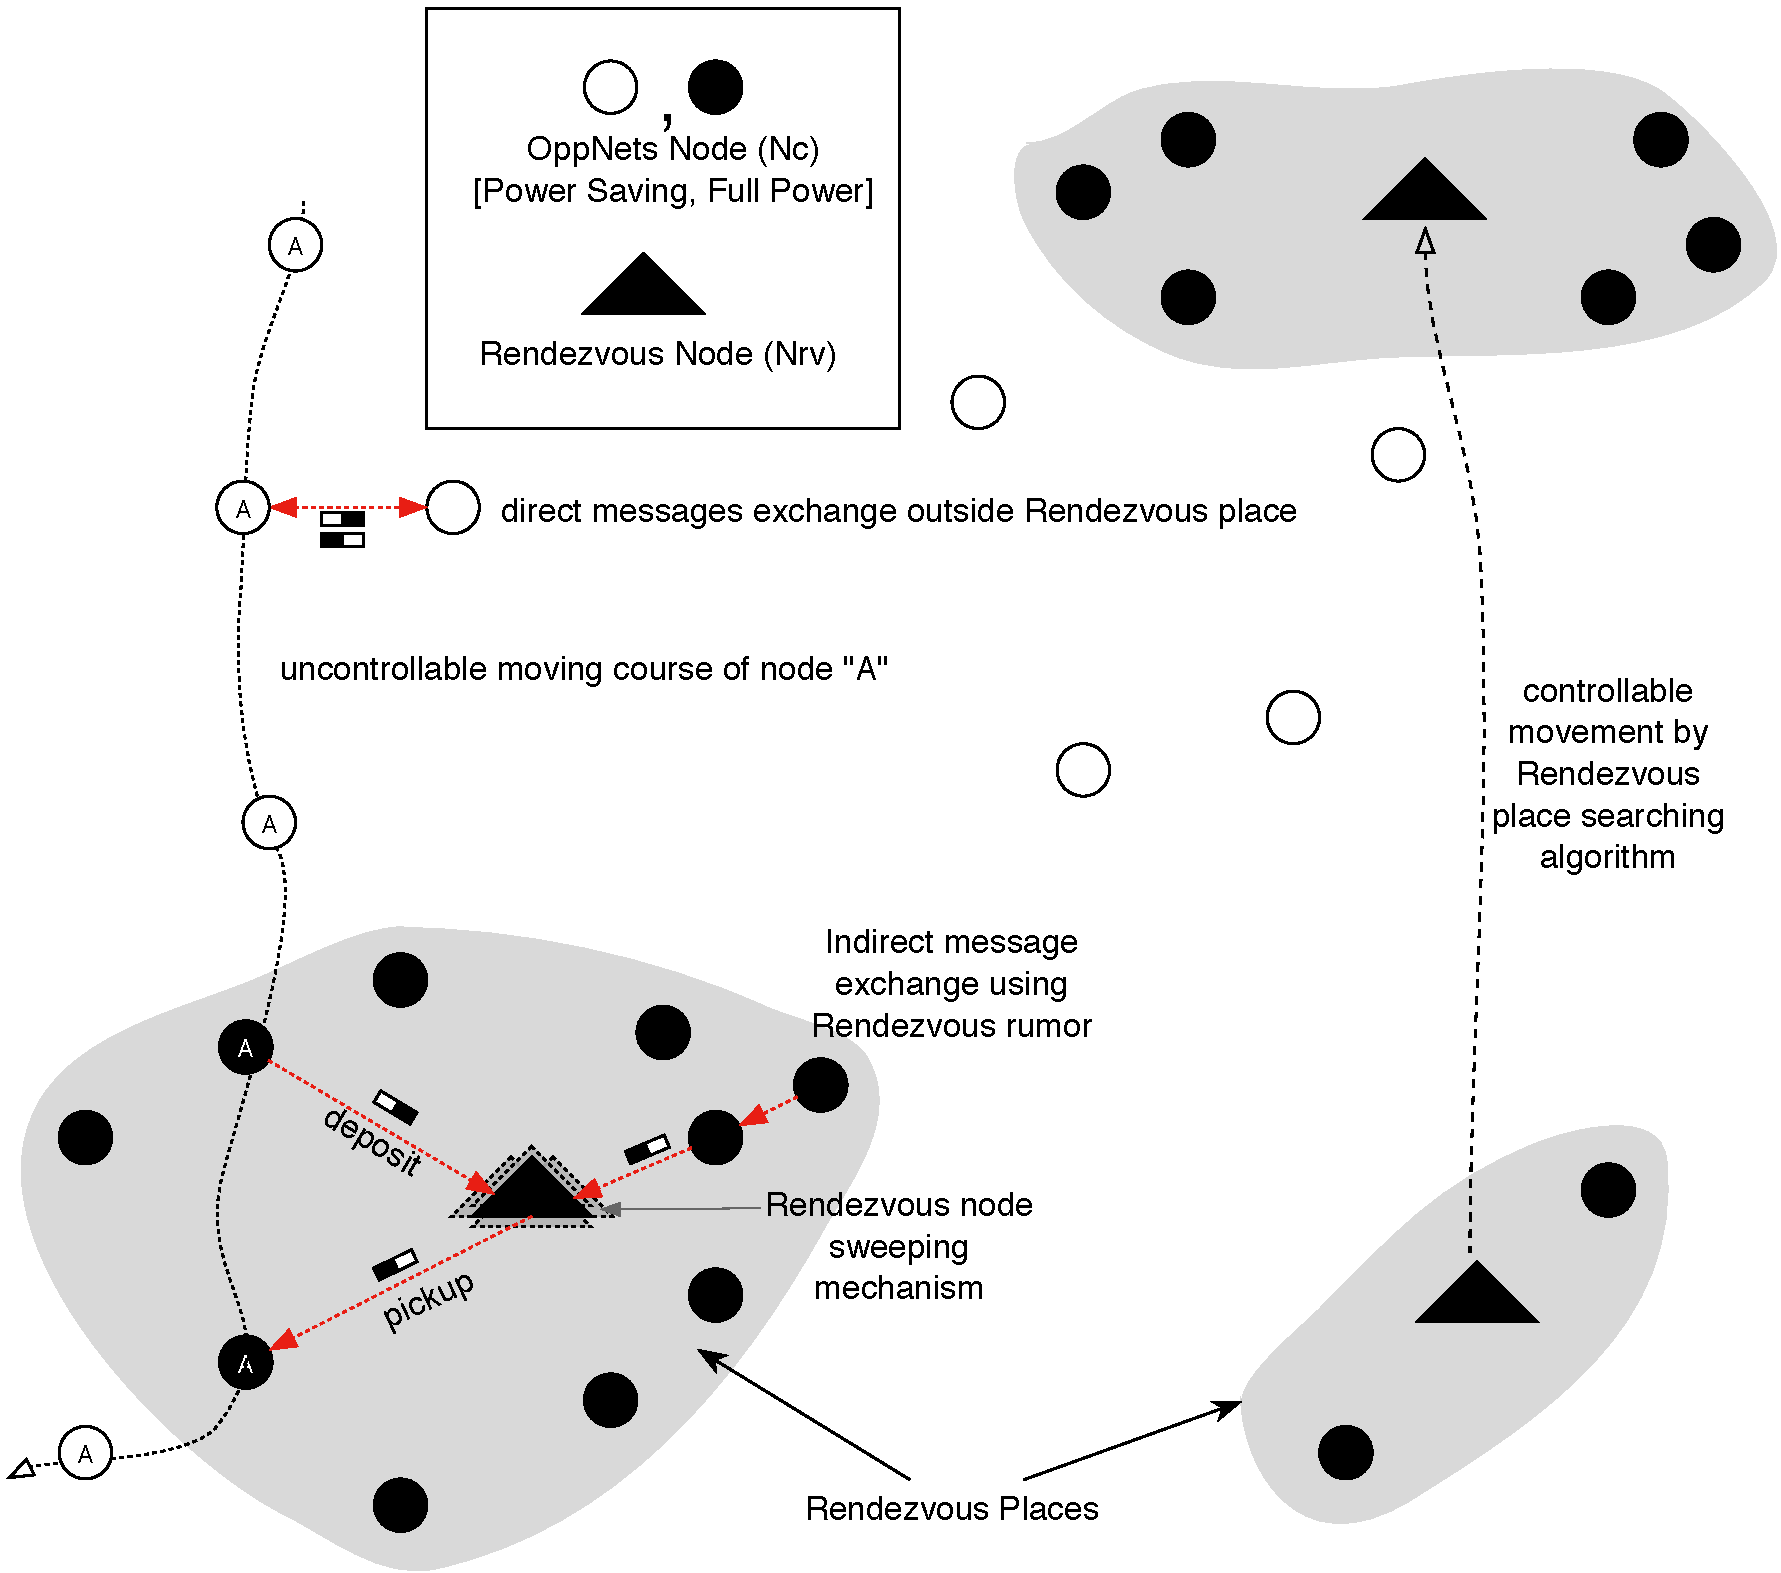
\includegraphics[width=5.5in]{Figures/NewSystemModel.pdf}
	\caption{System model}
	\label{System model}
\end{figure*}

The proposed system is designed to efficiently use the node-gathering area, i.e. Rendezvous place, for depositing the delivered messages as much as possible so that the messages can be picked up by the destination node without requiring the exact timing of direct contact between the node carrying a message and the desired destination node.
In addition, all nodes should reserve its energy as much as possible when they are out of the Rendezvous area.

As shown in Fig. \ref{System model}, the OppNet node, $N_{c}$, whose movement direction is uncontrollable, moves in the system using \textit{Power Saving Mode}  until it reaches the Rendezvous place where it will turn itself to \emph{Full Power Mode} in order to announce its arrival, deposit its carried messages and pick up the messages destined to itself, to/from the Rendezvous place.
The Rendezvous Rumor protocol and Rendezvous Node Sweeping mechanism are used inside the Rendezvous area to let messages being exchanged more effectively without the need of direct contact between the OppNet node and the high-resource direction-controllable Rendezvous node, $N_{rv}$, which is act as the center of the Rendezvous place.
The Rendezvous nodes will move around the OppNet network to create suitable Rendezvous places according to the proposed \emph{Rendezvous Place Searching algorithm}.

\subsection{OppNet node's operational modes: "Full Power" and "Power Saving"}
The OppNet node ($N_{c}$) is a mobile node equipped with the radio interface whose transmission rage is adjustable in range of $[{ r }_{ c }^{ min },{ r }_{ c }^{ max }]$.
The node will operate in either \emph{Full Power mode} or \emph{Power Saving mode} according to its location.
\subsubsection{Full power mode}
In this mode, the node will use its full transmission power, ${ r }_{ c }^{ max }$, to search for nearby nodes and exchange messages.
It will switch to this mode only when getting into the Rendezvous area.

\subsubsection{Power saving mode}
The node, by default, operates in this mode if it is outside the Rendezvous place.
In this mode, it will alternately change its transmission range between ${ r }_{ c }^{ min }$ and ${ r }_{ c }^{ max }$ in the process of searching for nearby nodes.
However, if it receives the searching signal from the other node, it will switch to its full ${ r }_{ c }^{ max }$ immediately in order to increase opportunity to exchange messages with the encountered node as much as possible.
Then, it will switch back to minimum ${ r }_{ c }^{ min }$ when departing from the communicating node.
Besides the ${ r }_{ c }^{ min }$ and ${ r }_{ c }^{ max }$ values, the ratio of the time interval being in it full ${ r }_{ c }^{ max }$ over the whole time period is a configurable parameter,$\tau_{s}$ , as shown in Fig. \ref{Operational modes}.

\begin{figure}[!t]
	\centering
	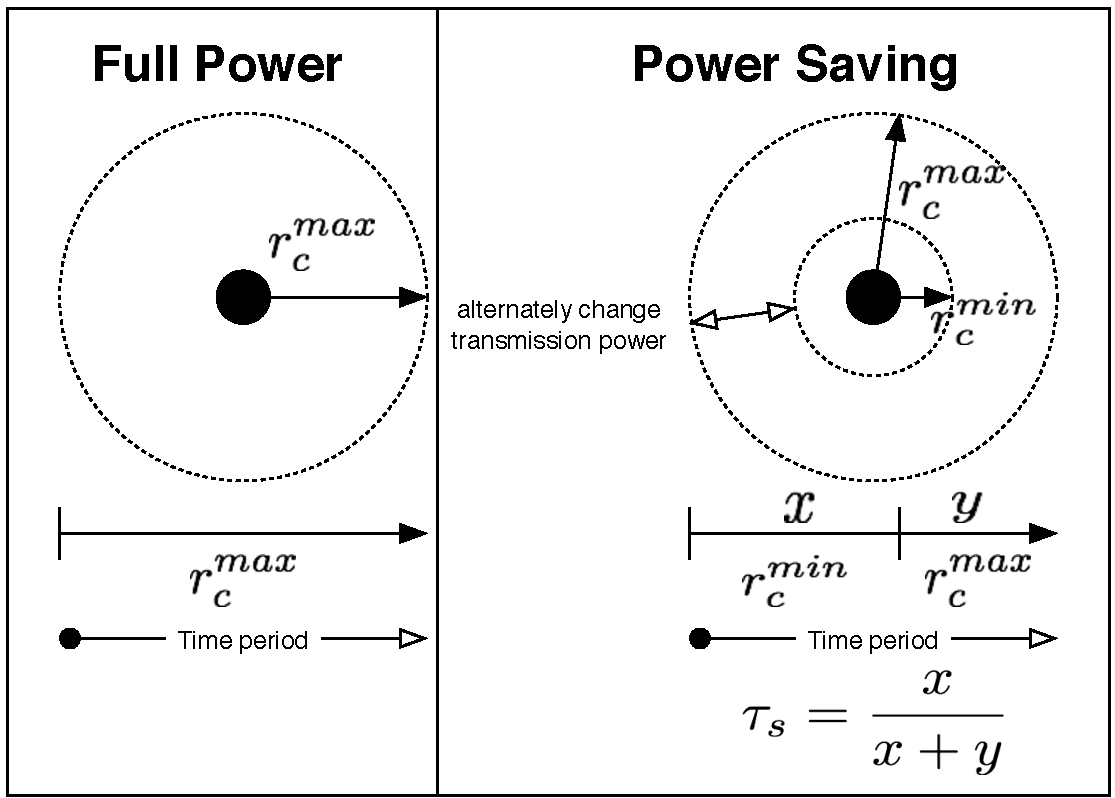
\includegraphics[width=3in]{Figures/OperationalMode.pdf}
	\caption{Operational modes}
	\label{Operational modes}
\end{figure}



\subsection{Rendezvous place and its Rumor protocol}

The Rendezvous place is a dynamic area centered by a special controllable Rendezvous node, $N_{rv}$.
This $N_{rv}$ node is full of resources such as large message storage and high radio power with maximum transmission range $R_{rv}$.
The Rendezvous place is controlled by the Rendezvous node using Rendezvous rumor protocol.

The area in Rendezvous place is not fixed as the maximum radio range, $R_{rv}$,  of the Rendezvous node, instead it is virtually determined by the covering radio range of the most outer OppNet nodes which can relay the data messages from the Rendezvous node, as shown in Fig. \ref{System model}

When an OppNet node detects the \emph{Rendezvous Area rumor message} $(RA)$ broadcasted from the Rendezvous node, it learns that it enters to the Rendezvous area.
Then, it will switch its operational mode to \emph{Full Power mode} and try to rebroadcast such \emph{Rendezvous Area }rumor message so that the other reachable nearby nodes can learn about Rendezvous place and can adaptively expand the area on-demand.
Additionally, the OppNet node in the Rendezvous area will periodically announce its arrival and upload its carried data messages to the Rendezvous node via the \emph{Keep-Alive} rumor message $(KA)$ and the \emph{Deposit} rumor message $(DP)$ respectively.
Note that all types of rumor messages will be automatically repeated with \emph{duplication filtering} function throughout the area by other OppNet nodes.

Once the rendezvous node receives the \emph{Keep-alive} rumor message which contains the sending node ID, it will gather all data messages destined to the node ID from its message storage, encapsulate those found messages into the created \emph{Pick-up} rumor message and then broadcast the \emph{Pick-up} message $(PU)$ throughout the Rendezvous area.
On the other hand, the Rendezvous node will keep all of data messages contained in the received \emph{Deposit} rumor messages in its storage for later sending out to the area when the target node appears later as seen in Fig. \ref{Rendezvous Place}. 

In addition to the Rendezvous rumor protocol, the Rendezvous node implements the rumor message sweeping algorithm in order to increase the chance to collect as many rumor messages as possible.
Instead of always being stationary at the center location of the Rendezvous place, the rendezvous node will periodically move to its four directions (North, East, West, South) by the distance of its radio transmission range as shown in Fig. \ref{Sweep mechanism}.
This design lets the OppNet nodes on the edge of Rendezvous node's radio range, whose radio signal may not reach to the Rendezvous node due to the difference in their radio transmission range, can speak back to the Rendezvous node.

\begin{figure}[!t]
	\centering
	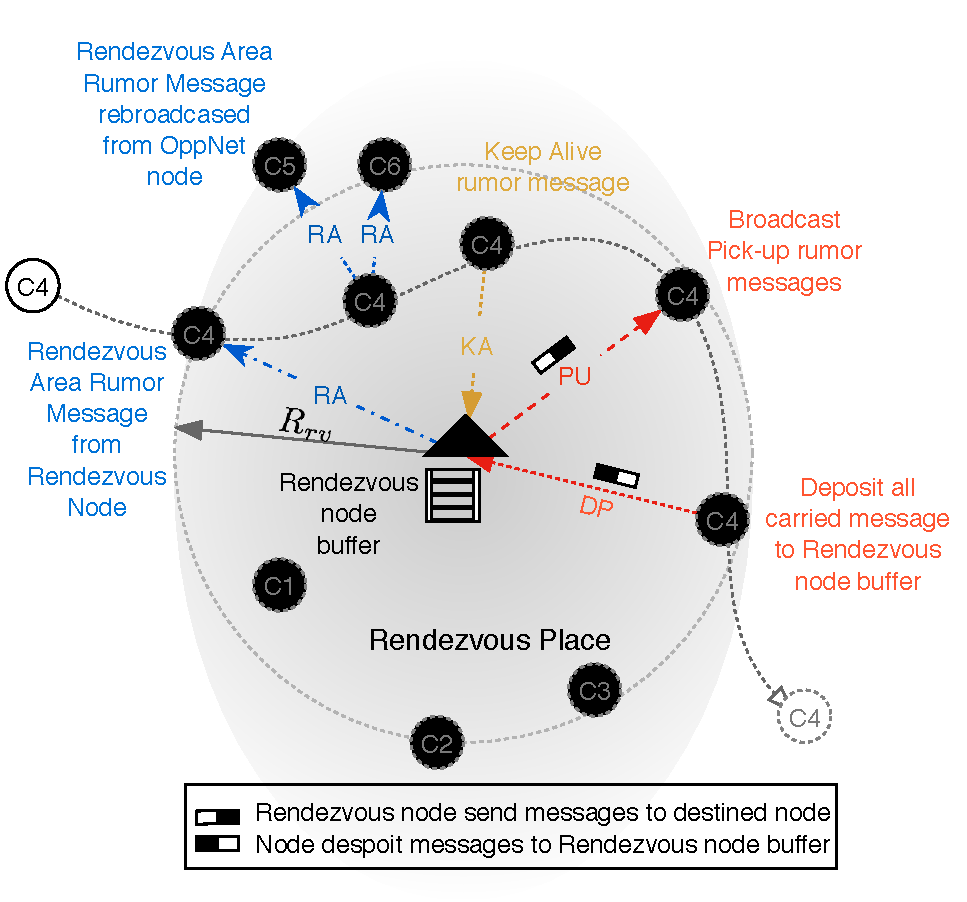
\includegraphics[width=3.5in]{Figures/NewRendezvousPlace.pdf}
	\caption{Rendezvous Place}
	\label{Rendezvous Place}
\end{figure}


\begin{figure}[!t]
\centering
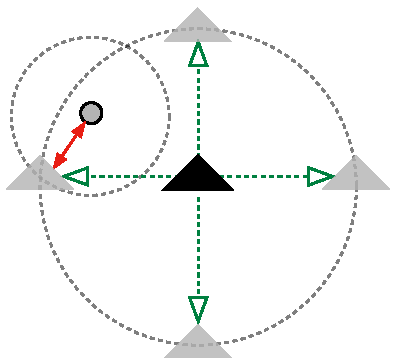
\includegraphics[width=1.5in]{Figures/Sweep.pdf}
\caption{Sweep mechanism}
\label{Sweep mechanism}
\end{figure}

\subsection{Rendezvous place searching algorithm}
In the proposed system, the Rendezvous node should move to find the node-gathering area corresponding with the real behavior of OppNet node.
\begin{figure}[!t]
	\centering
	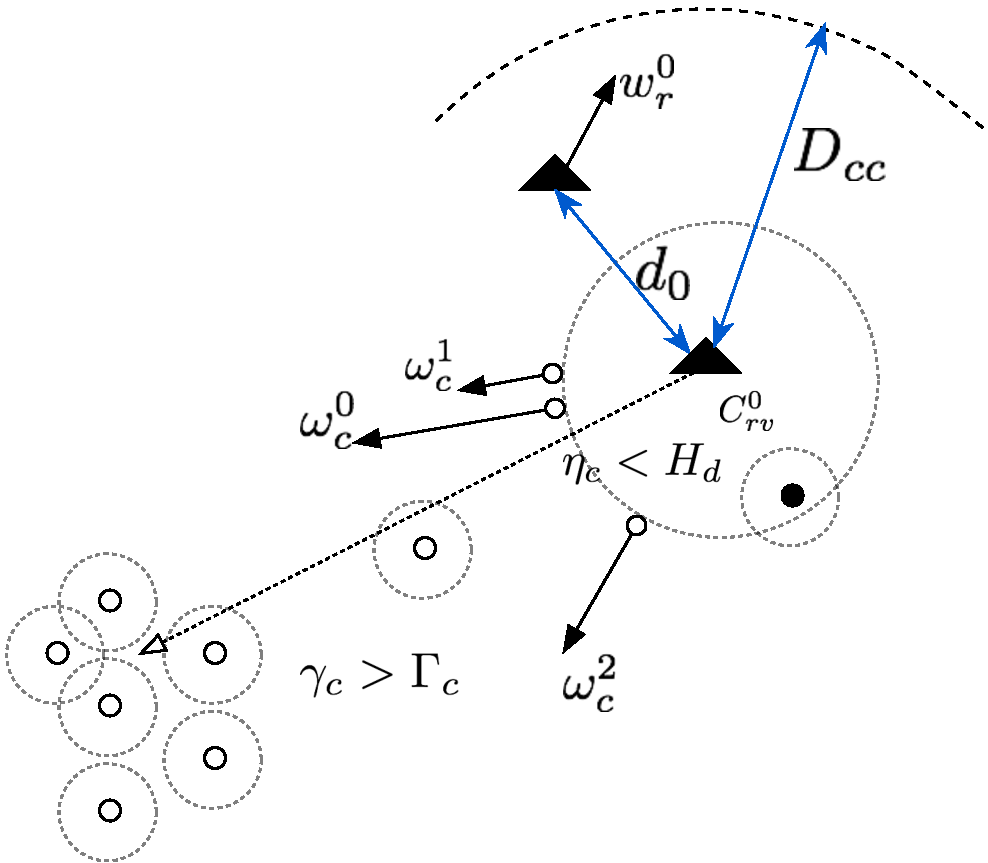
\includegraphics[width=2.5in]{Figures/Dynamic.pdf}
	\caption{Rendezvous place searching}
	\label{Rendezvous node movements}
\end{figure}
\subsubsection{Predictable behavior OppNet nodes}
In some applications, the movement of OppNet node is somehow predictable.
Take a wildlife monitoring as an example, most animals are usually cyclically gathering in the high supplies area such as along side of the main river of some specific place at some specific time \cite{Yu2007}.
In these applications, the Rendezvous nodes can be programmed to be located at those areas at the proper time in order to maximize the effectiveness of the proposed system.

\subsubsection{Non-Predictable behavior OppNet nodes}
Without any priori knowledge about OppNet node, the proposed \emph{dynamic Rendezvous Place Searching Algorithm} can be used to guide the Rendezvous nodes to the node-gathering area.
The Rendezvous node will decide to move to the new node gathering location if the number of OppNet node in the current Rendezvous place ($\eta_{c}$) falls below the predefined departure node threshold, $H_{d}$.
The movement direction, $\vec{\Delta}$, will be determined periodically based on the collected statistical data from both previously contacting OppNet nodes and other neighboring Rendezvous nodes as in Eq.\ref{DirectionParameter}.
In the equation, $\vec{w_c}$ is the departure directional unit vector of the contacted OppNet nodes, $\vec{w_r}$ is the directional unit vector of the other Rendezvous nodes and the $\varphi$ is a configurable weighting factor between group of OppNet nodes and group of other Rendezvous nodes in the area.

\begin{eqnarray}
\label{DirectionParameter}
\vec{\Delta} =\sum _{ i=1 }^{ C }{ \vec { { \omega }_{ c }^{ i } }  } + \varphi \sum _{ j= }^{ R }{ \delta\left( d_{j} \right)
	\vec { {w }_{ rv }^{ j } }  }
\end{eqnarray}

While the $\delta\left( d_{j} \right)$ is the on-off function to include only the other Rendezvous nodes whose distance $d_j$ is the range of cut-off distance perimeter, $D_{cc}$, and the  $C$ and $R$ are the number of contacted OppNet nodes and the number of other Rendezvous nodes respectively.

\[\delta \left( { d }_{ j } \right) =\begin{cases} 1\quad ;\quad { d }_{ j }\quad \le { \quad D }_{ cc } \\ 0\quad ;\quad { d }_{ j }\quad >{ \quad D }_{ cc } \end{cases}  \] 

The Rendezvous node will decide to stop at the expected node-gathering area when the number of OppNet nodes in the current Rendezvous place ($\gamma_{c}$) become greater than the predefined Rendezvous place node threshold, $\Gamma_{c}$ as shown in Fig. \ref{Rendezvous node movements}.  


\section{Evaluation}
The objective of the evaluations is to analyze the performance of our proposed protocol on the sparse network environment comparing with traditional OppNet protocols.
We compare both predictable and non-predictable behavior OppNet nodes with the commonly well-known Epidemic protocol\cite{Vahdat2000} under different node density environments.


\subsection{Simulation setup}
We setup a simulation environment using ONE (Opportunistic Network Environment) \cite{Keranen2009b}, which is a powerful tool designed for running opportunistic network simulation with various routing protocols and different movement models.
All the results are obtained by averaging over a few hundreds independent simulation runs with different seeds.
For the OppNet simulation model, the main parameter that largely effected the evaluation performance is the movement model.
In our evaluation, we deploy Group movement model instead of the most commonly used, Random Way Point (RWP) model \cite{Batabyal2012}, to correctly capture the the actual behavior of node movements.
In fact, several multi-hop wireless network scenarios are most realistically represented using Group movement model \cite{Blakely2004} which represents the random motion of a group of mobile nodes as well as the random motion of each individual mobile node within the group.
This is the vital case for modeling the routing simulation in OppNet since the movements in several cases are in swarm behavior, in which nodes are aggregates together and moving in some directions, such as the movement of animals or military tactical operations.
The other parameters that mainly effect the evaluation performance are the area of operation, the wireless range of the nodes, node velocity and spatial location of the nodes \cite{Batabyal2012}. 
In our simulation, we fix the number of nodes while increasing and decreasing the area of operation which results in wide range of node density parameter for evaluation.
Node density ($\lambda$) is defined as the number of nodes per unit area. 
If $N$ nodes are distributed in a square grid of size $M \times M \quad{ m }^{ 2 }$ then the $\lambda$ is given by $\lambda =\frac { N }{ { M }^{ 2 } } $ . 
The wireless range of our OppNet node can be adjusted depending on the environment while the node velocity is equal to the normal human walking speed.
The common parameters are summarized in Table \ref{table_parameters}.

\subsection{Metric}
\begin{table}[!t]
	\renewcommand{\arraystretch}{1.3}
	\caption{simulation variables}
	\label{table_parameters}
	\centering
	\begin{tabular}{|c|c|c|}
		\hline
		Parameters         &  $N_{c}$ & $N_{rv}$ \\ \hline
	%	Simulation Time     & \multicolumn{2}{|c|}{10800 Seconds }  \\ \hline
		Message Size       &  \multicolumn{2}{|c|}{500 KB - 1 MB}        \\ \hline
		% Node Buffer         & \multicolumn{2}{|c|}{500 MB}&  10 GB      \\ \hline
		Maximum Radio Range & 30 Meters  & 100 Meters \\ \hline
		Transmission Speed &  \multicolumn{2}{|c|}{ 54 Mbps   }        \\ \hline
		Router             & \multicolumn{2}{|c|}{ DRRA | Epidemic   } \\ \hline
		Moving Speed       &   \multicolumn{2}{|c|}{0.5 - 1.5 m/s }        \\ \hline
		Movement Model     &   \multicolumn{2}{|c|}{Group Movement Model  }      \\ \hline
	\end{tabular}
\end{table}
Opportunistic routing protocols are commonly evaluated by delivery ratio, median latency and network overhead.
However, we required specific composite metrics in order to clearly observe the performance of our proposed protocol. 
In our evaluation we consider the following metrics:

	\paragraph{Delivery ratio ($D_{r}$)} is defined as the ratio of the total number of messages successfully delivered within the deadline ($ { M }_{ delivered }$) to the total number of messages created from the source nodes that need to be delivered ($ { M }_{ created }$) as shown in Eq. \ref{delivery_ratio}.
	\begin{equation}
	\label{delivery_ratio}
	D_{r} =\frac { { M }_{ delivered } }{ { M }_{ created } } 
	\end{equation}

\paragraph{Delivery performance ($D_{p}$)} is a composite metrics defined as a delivery ratio per energy consumption unit in order to clearly analyze our protocol performance.
Basically, the relation between energy consumption and radio range can be determined by Eq.\ref{eq:enegy} \cite{Yang2010, Wang2006}.

\begin{IEEEeqnarray}{rCl}
	\label{eq:enegy}
	{ E }_{ T }\quad =\quad L\cdot  { \epsilon  }_{ fs } \cdot  { d }^{ \alpha  }
\end{IEEEeqnarray} 

${ E }_{ T }$ is the amounts of transmission energy consumed at a node for transmitting an L-length message, where $\alpha$ is the power loss component with $\alpha \in \left[ 2,4 \right]$ and $\epsilon { f }_{ s }\left[ J/(bit/{ m }^{ \alpha  }) \right]$ is the amount of energy consumed by an amplifier to transmit one bit data at an acceptable quality level.
In this protocol, we approximately determine the relationship between unit of consumed energy and radio radius of node in the term of exponential equation.
We assume the simplicity of energy model by only accounting for the communication energy consumption of a wireless interface and do not consider other resources such as computation, location services or mobility.
In fact, the messages generated from protocol are accounted for the delivery performance.
As a result, the energy consumption can be simply derived as Eq. \ref{eq:new_energy}.

\begin{eqnarray}
	\label{eq:new_energy}
	{ E }_{ P }\quad \propto { \quad M }_{P }\cdot{ r }_{ P }^{ 2 }
\end{eqnarray}

Therefore, the delivery performance can be calculated from  Eq. \ref{eq:delivery_performance}.

\begin{eqnarray}
\label{eq:delivery_performance}
{ D }_{ P }=\frac { { D }_{ r }^{ P } }{ { E }_{ P,B } } =\frac { { D }_{ r }^{ P } }{ \left( \frac { { M }_{ P }{ \cdot r }_{ P }^{ 2 } }{ { M }_{ B }\cdot { r }_{ B }^{ 2 } }  \right)  } 
\end{eqnarray}

In this Equation, $P$ is the target protocol while $B$ is the baseline protocol (Epidemic protocol, for example) to be used as comparative energy reference.
$M$ is the message number transmitted by OppNet nodes, excluding Rendezvous node in Rendezvous place.
The average transmission radius is referred as $r$ while $\alpha$ is the power consumption exponent factor [2,4] which we are using the value of 2 for our simulation.


\subsection{Simulation Results}


This section shows the results of the different simulations that have been performed evaluating the impact in the performance.
The following subsections include the results of each set of simulations.

\subsubsection{Delivery performance}

\begin{figure}[!t]
	\centering
	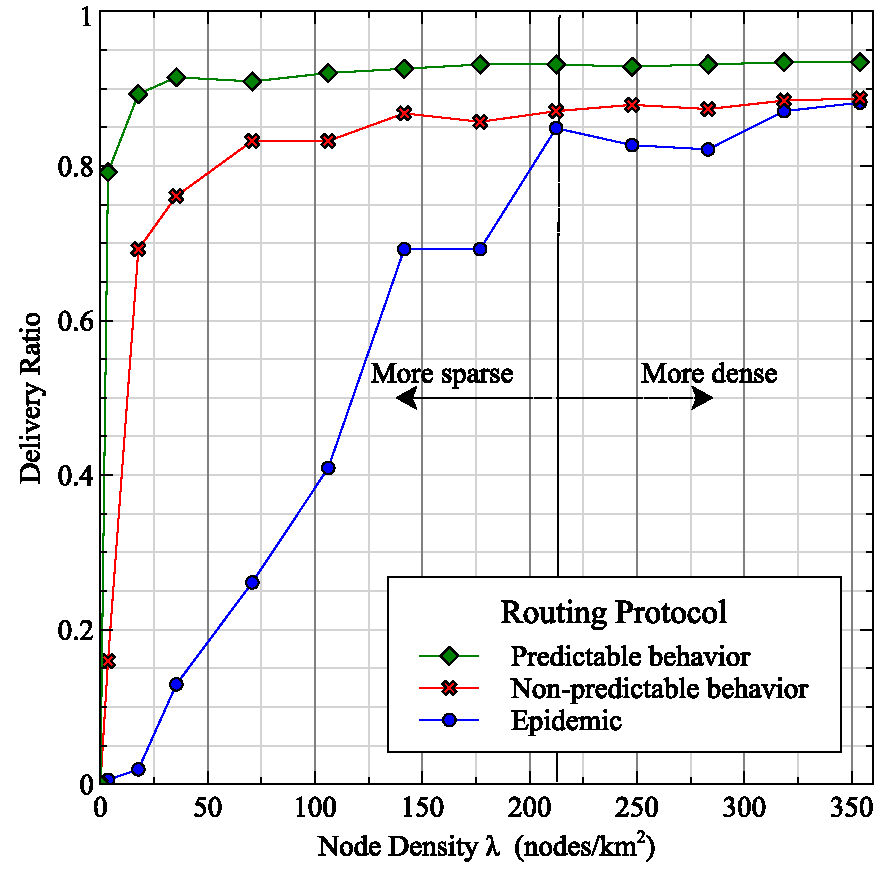
\includegraphics[width=2.5in]{Graphs/DeliveryRatio.pdf}
	\caption{Delivery Ratio per Node Density}
	\label{Delivery Ratio per Node Density}
\end{figure}

\begin{figure}[!t]
\centering
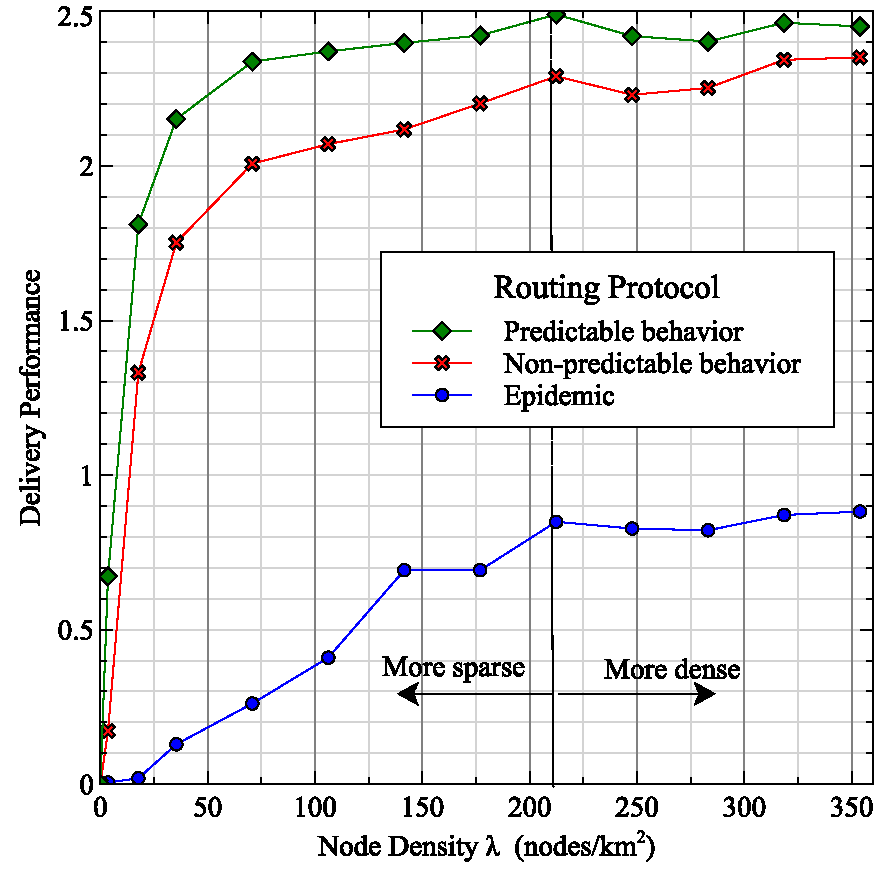
\includegraphics[width=2.5in]{Graphs/NetworkPerformance.pdf}
\caption{Delivery Performance per Node Density}
\label{Network Performance per Node Density}
\end{figure}

Firstly, the comparison of delivery ratio is shown in Fig. \ref{Delivery Ratio per Node Density} while $x-axis$ represents the node density (the number of nodes in the area of 1 $km^2$) and $y-axis$ shows the delivery ratio.
In our simulation, we assume the environment with 1 Rendezvous node and the ratio of time interval factor between full power and power saving, $\tau_s$ of 0.5.

Fig. \ref{Delivery Ratio per Node Density} shows that our proposed protocols gain slightly better delivery ratio in the dense environment.
On the other hand, the proposed protocols gain significantly higher delivery ratio in the sparse environment by maintaining the ratio up to 80\%, even when node density is as low as 50 $nodes/km^2$ in non-predictable behavior or as low as 5 $nodes/km^2$ nodes in predictable behavior.
Over all in average, our proposed protocols gain approximately 40\% higher delivery ratio than existing traditional Epidemic routing.

The reason behind the behaviors from this result is that the Rendezvous concept can be clearly performed better when the node density becomes sparse since all nodes can effortlessly exchange messages in the dense network.
However, in the sparse network, the Rendezvous nodes can help facilitating the messages exchange mechanism among OppNet nodes which resulting in much higher delivery ratio.
In addition, with the knowledge of node gathering-area, the delivery ratio can be further increased especially in the extremely low node density.

Furthermore, the proposed protocols utilize less energy consumption which is a vital factor in opportunistic network because the mobile nodes in this scheme are usually equipped with limited power resources that the performance can be seen in Fig. \ref{Network Performance per Node Density}.
Similar to graph of delivery ratio, we compare the delivery performance ($y-axis$) on node density ($x-axis$), in which the $D_p$ can be calculated from Eq. \ref{eq:delivery_performance}.
It can be obviously seen that the proposed protocols in Fig. \ref{Network Performance per Node Density} can save about half of energy consumption in order to achieve the same delivery ratio in the dense environment.
Nevertheless, the propose protocol use only 25\% power consumption in sparse environment.
The better delivery performance results from the lower messages number of our proposed protocols compare to the Epidemic counter part as can see in Fig. \ref{Number of Created Messages per Node Density}.
Additionally, the other factor that impact the higher delivery performance is the lower average wireless transmission of our proposed protocol.

\begin{figure}[!t]
	\centering
	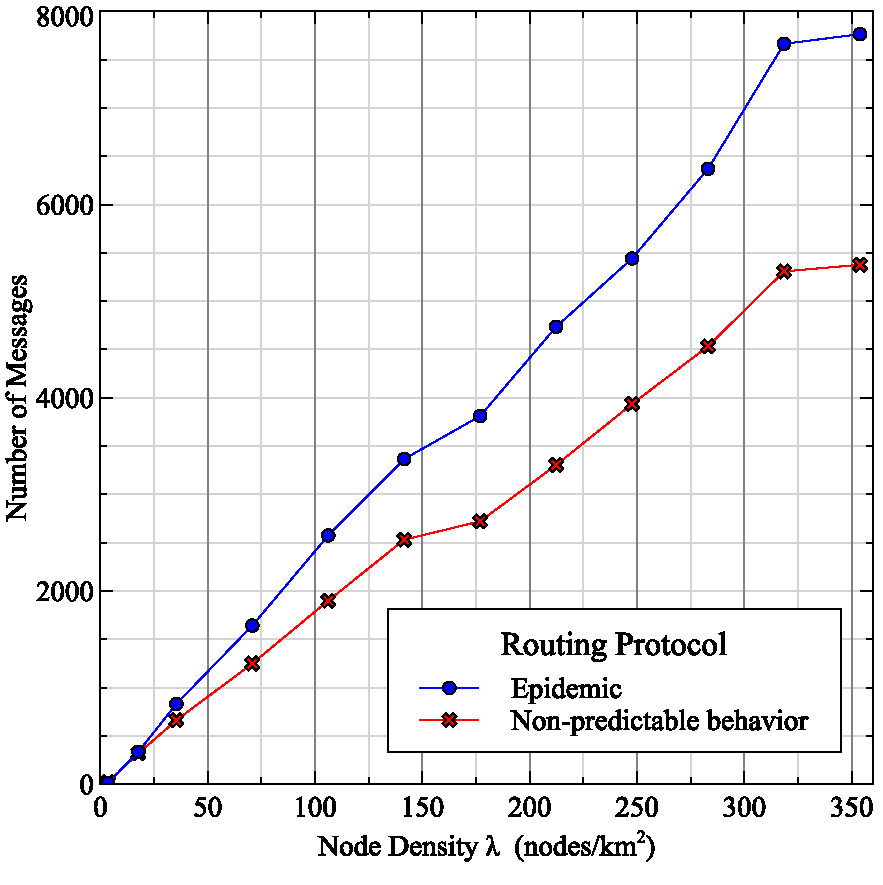
\includegraphics[width=2.5in]{Graphs/messages.pdf}
	\caption{Number of Created Messages per Node Density}
	\label{Number of Created Messages per Node Density}
\end{figure}

\subsubsection{Power saving factor}
% \begin{figure}[!t]
% 	\centering
% 	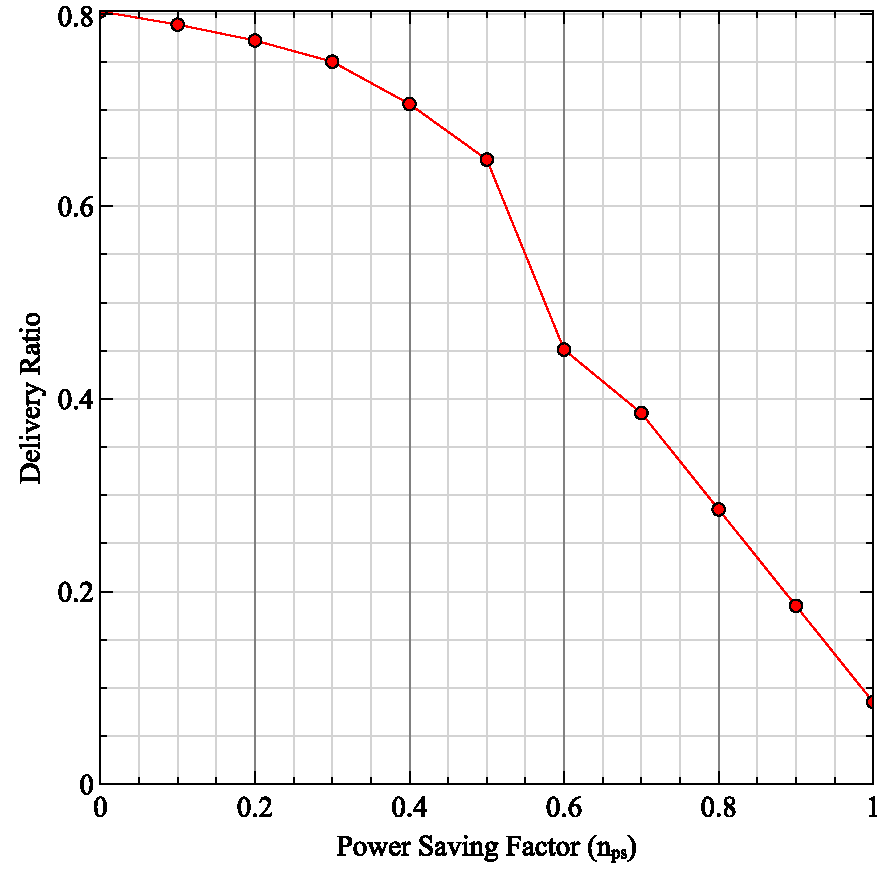
\includegraphics[width=2.5in]{Graphs/NpsDelivery.pdf}
% 	\caption{Delivery Ratio per Power Saving Factor}
% 	\label{Delivery Ratio per Power Saving Factor}
% \end{figure}

% \begin{figure}[!t]
% \centering
% 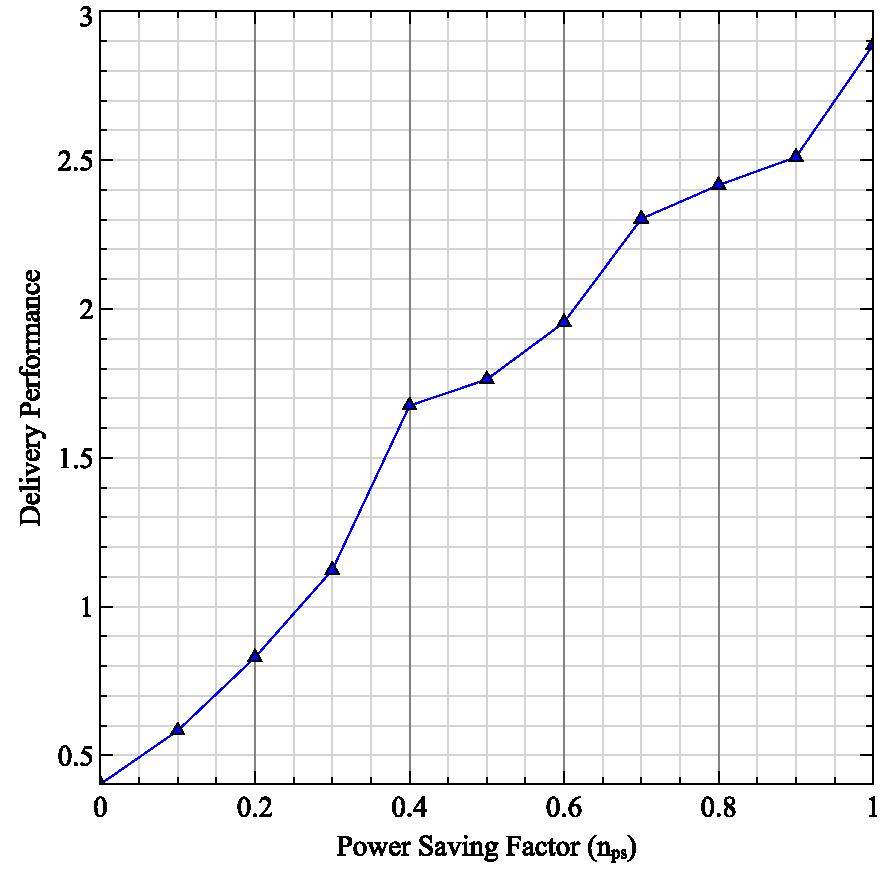
\includegraphics[width=2.5in]{Graphs/NpsDeliveryPerformance.pdf}
% \caption{Delivery Performance per Power Saving Factor}
% \label{Delivery Performance per Power Saving Factor}
% \end{figure}

In this section, we study the factors effecting the power saving and the trade-off between power consumption and delivery ratio.
%%
We define the Power Saving Factor, $n_{ps}$ as the energy consumption parameter to analyze the power utilization of our proposed protocol which can be determined as in Eq. \ref{nps}.
%%
In the simulation, we select the density of 100, 200 and 300 nodes to study the impact of power saving factor to the delivery ratio on different density envioronment.

\begin{equation}
{ n }_{ ps }={ \tau  }_{ s }\cdot \frac { { r }_{ c }^{ max }-{ r }_{ c }^{ min } }{ { r }_{ c }^{ max } } 
\label{nps}
\end{equation}

\begin{figure}[!t]
\centering
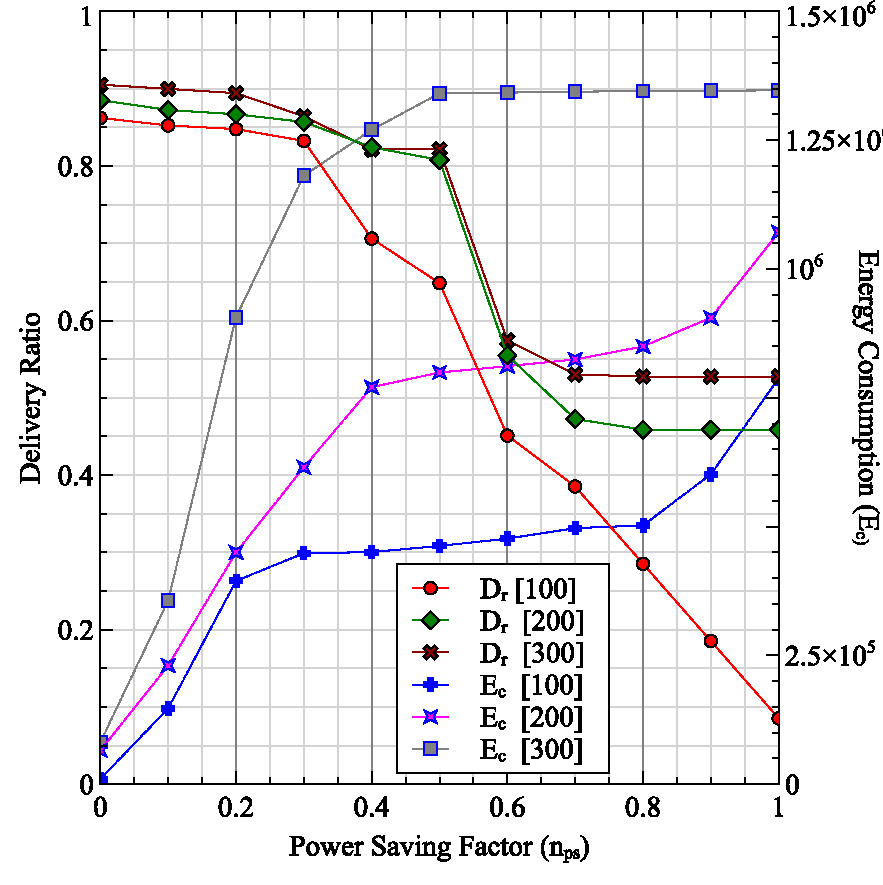
\includegraphics[width=2.5in]{Graphs/NpsDeliveryPerformanceAndDeliveryRatio.pdf}
\caption{The Optimum between Delivery Ratio and Delivery Performance}
\label{The Optimum between Delivery Ratio and Delivery Performance}
\end{figure}

From Fig. \ref{The Optimum between Delivery Ratio and Delivery Performance}, the graph presents the declining in the delivery ratio when the value of $n_{ps}$ increases.
%%
This implies that in the attempt of saving the energy, the deliverable of messages are effected from the wireless range reduction.
%%
On the other hand, the delivery performance is increasing with the value of power saving factor which shows that the higher the $n_{ps}$, the higher the delivery performance.
%%
Overall, the key point of Fig. \ref{The Optimum between Delivery Ratio and Delivery Performance} is the cross point between delivery ratio and delivery performance which can see at $n_{ps} = 0.55$ which is the optimum point of our method.



% Fig. \ref{Delivery Ratio per Power Saving Factor} shows the effect of power saving factor on delivery ratio.
% %%
% This graph presents the declining in the delivery ratio when the value of $n_{ps}$ increases.
% %%
% This implies that in the attempt of saving the energy, the deliverable of messages are effected from the reduce in the wireless range.
% %%
% However, the delivery performance is increasing with the power saving factor as seen in Fig. \ref{Delivery Performance per Power Saving Factor}.
% %%
% This result illustrates that in order to gain higher delivery performance, the power saving factor is also increasing.



% As a result, the trade-off between the delivery ratio and delivery performance is shown in Fig. \ref{The Optimum between Delivery Ratio and Delivery Performance}.
% From the graph, the optimum is on the power saving factor of 0.6




% In this section, we study the factors effecting the power saving of the proposed protocols by analyzing the impact of $\tau_s$ on the delivery performance as seen in Fig. \ref{Utilization ratio of wake-up interval comparison}.
% This graph varies the ratio of $\tau_s$ which is the time interval of $r_c^{min}$ over overall period, starting from 0.1 to 1.0. 
% Additionally, Fig. \ref{Network performance per ratio range ratio} presents the delivery ratio of non-predictable Rendezvous routing over the radio range ratio, varying from 0.1 to 1.0. 
% This radio range ratio ($R_s$) is defined by ${{ r }_{ c }^{ min }}/{{ r }_{ c }^{ max }}$ which is the minimum radio range per maximum range of the OppNet nodes.

% The result from Fig. \ref{Utilization ratio of wake-up interval comparison} shows that the value of $\tau_s$ varies directly to the delivery performance, which suggests that keeping the state of  operation in saving mode longer resulting in higher $D_p$.
% Similarly, the delivery ratio from Fig. \ref{Network performance per ratio range ratio}  is increased with the higher of radio range ratio which means increasing the ${ r }_{ c }^{ min }$ will result in higher delivery ratio.
% Therefore, to increase the delivery performance, we have to escalate the value of $\tau_s$ and $R_s$ which means maintaining the operation of power saving mode as long as possible while extending the ${ r }_{ c }^{ min }$.
% The reason behind this result comes from Eq. \ref{eq:delivery_performance}, in which the value of radio range is the leading factor effecting the delivery performance.
% In parallel, the time period of ${ r }_{ c }^{ min }$ state is effecting the value of $D_p$ since the result shows that the delivery performance varies directly to the $\tau_s$.

\subsubsection{Rendezvous node factor}
\begin{figure}[!t]
	\centering
	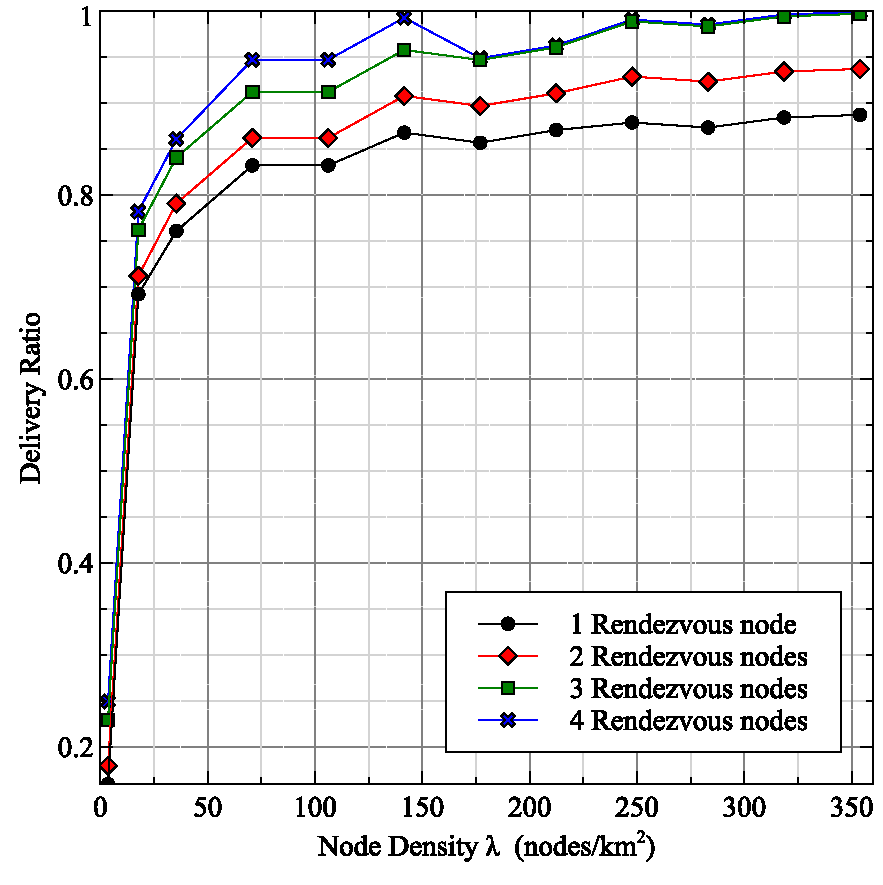
\includegraphics[width=2.5in]{Graphs/MultipleRVs.pdf}
	\caption{Multiple Rendezvous Nodes}
	\label{Multiple Rendezvous Nodes}
\end{figure}
\begin{figure}[!t]
\centering
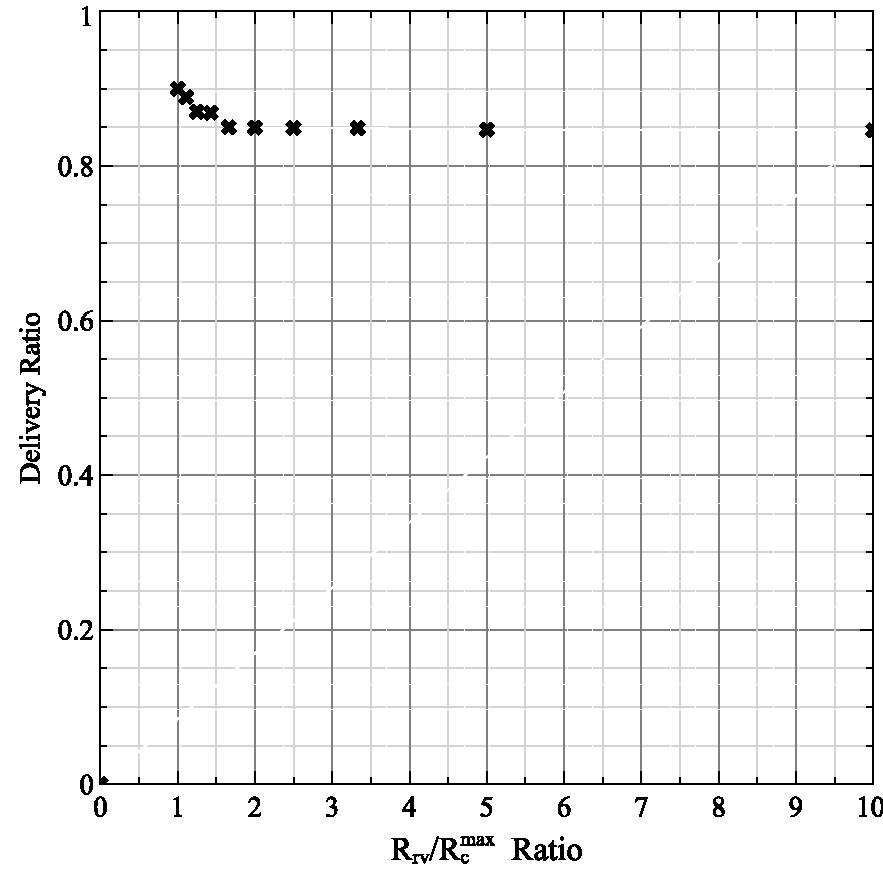
\includegraphics[width=2.5in]{Graphs/RcmaxRrv.pdf}
\caption{$R_c^{max}/R_{rv}$ ratio}
\label{$R_c^{max}/R_{rv}$ ratio}
\end{figure}
We investigate the main parameters effecting the environment of $N_{rv}$ in this part.
In Fig. \ref{Multiple Rendezvous Nodes}, the number of $N_{rv}$ are varied from one to four nodes in our simulation.
The result shows similar trend of overall delivery ratio which slightly declining when the node density decreases.
Nevertheless, the delivery ratio increase when more rendezvous nodes are injected into the environment.
The results suggest that more number of rendezvous node can gain higher delivery ratio.
Fig. \ref{$R_c^{max}/R_{rv}$ ratio} shows the relationship between $R_c^{max}$ and $R_{rv}$ over the delivery ratio, starting from  $R_c^{max}/R_{rv}$ ratio of 0.1 to 1.0.
This graph shows moderate incrementing in delivery ratio when the ratio of $R_c^{max}/R_{rv}$ increases.
The result suggests that the value of $R_c^{max}$ has slightly effect on delivery ratio. 

%\subsubsection{Effect of time interval on operational modes}
%Since the key benefit of our protocol is the dynamic radio range, the trade off of energy consumption and delivery ratio requires to be analyzed.
%Fig. \ref{Utilization ratio of wake-up interval comparison} shows the delivery performance of each node density varying by $\tau_{s}$.
%The result clearly shows that the delivery performance increase with the value of $\tau_s$. 
%The value of $\tau_s$ = 1 can maximize the delivery ratio.
%This means that we should maximize the full-power mode as much as possible in order to gain better delivery ratio.
%As a result, the significance of wireless range is higher than energy minimizing time.

%\subsubsection{Impact on radio range ratio}
%We study the impact of radio range level ratio for OppNet nodes on delivery ratio as seen in Fig. \ref{Network performance per ratio range ratio}.
%This radio range ratio is defined by ${ r }_{ c }^{ min }/{ r }_{ c }^{ max }$ which is the minimum radio range of OppNet node per maximum range.
%The result suggest the increasing in delivery ratio when the radio range ratio increase especially at the exponential rate at the ratio of 0.1 to 0.6.
%However, after 0.6 ratio the delivery ratio slightly increases.
%This means that our protocol gain higher delivery ratio if we increase the ${ r }_{ c }^{ min }$.

%Rewrite the drawback
%\subsubsection{Average latncy}
%Fig. \ref{Average latency on node density} shows the delay of our routing protocol comparing to traditional Epidemic protocol varying by node density.
%From the graph, our Rendezvous protocol gain slightly higher average latency than Epidemic protocol especially at 350 $nodes/km^2$.
%This is a drawback of our protocol since the concept of smart node requires specific computation time in order to route the messages more efficiently. 
 
%\begin{figure}[!t]
%	\centering
%	\includegraphics[width=2.5in]{Graphs/latency.pdf}
%	\caption{Average latency on node density}
%	\label{Average latency on node density}
%\end{figure}

\section{Conclusion}
Opportunistic Routing techniques can be applied in  plentiful variety of scenarios such as military network or wildlife monitoring. 
In this paper, we investigate the use of rendezvous points in opportunistic network routing to increase the delivery ratio in extreme sparse network environment.
This novel protocol proposes the two new types of node, Rendezvous node and OppNet node, which can help maintaining the messages in one place as long as possible in order to bridge the gap of time and space domain.
In this Rendezvous place, the passing nodes can announce, deposit and pickup their own messages without meeting with other nodes that carried desired messages.
The size and shape of  Rendezvous place can be adapted to the environment of OppNet nodes in the area.
We define our routing model in two functions: predictable  and non-predictable behavior OppNet node functions.
The result suggest that our protocols perform significant higher in delivery performance which is the trade off of delivery ratio per energy consumption.
We can simply imply that if the location of rendezvous place can be predicted, we can achieve highest network performance.
Our experiment also suggest that the OppNet node can gain higher delivery performance when the time interval of power saving mode is longer and the minimum radio range is higher.
In the future work, this concept of smart node can be further extend to increase the intelligence of the node since the technologies are advanced rapidly.


\section*{Acknowledgment}
This work was supported by Sirindhorn International Institute of Technology, Thammasat University, Thailand and Basic Research Program from Data Communication Laboratory, Research and Development Department at Defense Technology Institute Thailand.

\bibliographystyle{IEEEtran}
\bibliography{RendezvousBib}
\end{document}


